\chapter{Premier pas dans un CTF}
\label{chap:BDD}

    Nous voici donc partis pour notre premier CTF. En général, l’adresse IP de la machine cible sera fournie mais au cas où ça ne serait pas le cas, nous vous conseillons d’utiliser un ‘arp-scan --localnet’ comme ceci :

%Image arp-scan
\begin{figure}[htp!]
  \centering
  \setlength\figureheight{7cm}
  \setlength\figurewidth{9cm}
  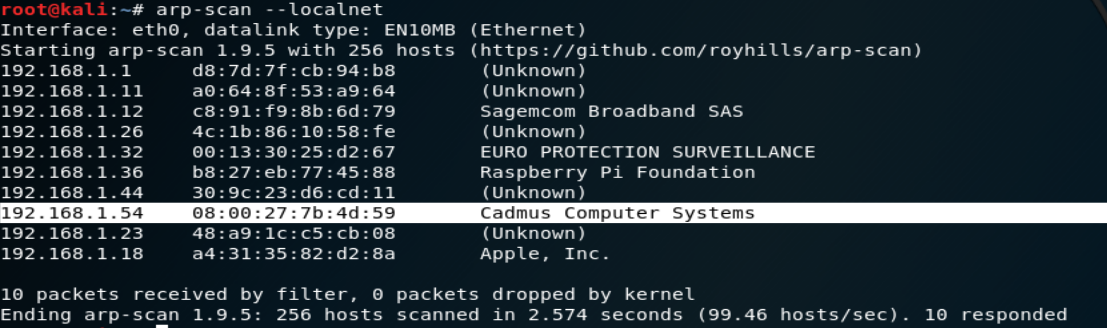
\includegraphics[width=1\textwidth]{oui/Screens/unknown.png}
  \caption{ARP-SCAN}
  \label{fig:courbe-tikz}
\end{figure}

Si la machine cible est connue sous un nom DNS, il est possible, soit de ping ce nom ou bien de réaliser un nslookup que nous allons privilégier. Comme on peut le voir ci-dessous, nous pouvons retrouver l'addresse IPV4 et IPV6 d'une machine connue sous son nom :

\begin{figure}[htp!]
  \centering
  \setlength\figureheight{7cm}
  \setlength\figurewidth{9cm}
  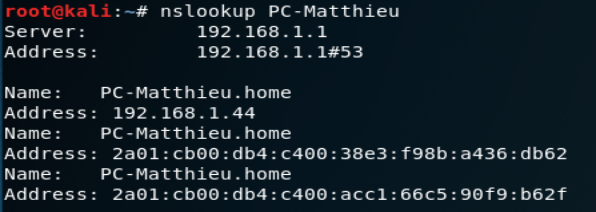
\includegraphics[width=0.6\textwidth]{oui/Screens/nslookup.PNG}
  \caption{Nslookup}
  \label{fig:courbe-tikz}
\end{figure}

\newpage
\section{ARP-Scan}
Arp-scan est un utilitaire qui permet  d’obtenir les adresses IP d’un réseau via la couche 2 du modèle OSI . Le modèle OSI est une norme d’exemple pour tous les types de transmissions réseaux. Ce modèle peut être vu de cette manière :
%Image modèle OSI
\begin{figure}[htp!]
  \centering
  \setlength\figureheight{7cm}
  \setlength\figurewidth{9cm}
  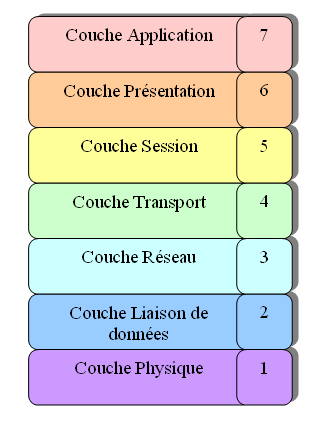
\includegraphics[width=0.3\textwidth]{oui/Screens/modeleOSI.PNG}
  \caption{Schéma du modèle OSI}
  \label{fig:courbe-tikz}
\end{figure}

La couche 2 est la couche de liaison de données. Cette dernière correspond à l’adressage physique des machines, soit l’adresse MAC. L’adresse MAC est l’adresse unique d’une interface réseau d’un équipement. Cette adresse est codée en hexadécimal en 6 octets.

\subsection{Fonctionnement d'ARP-Scan}

Ce dernier va envoyer une requête ARP en broadcast sur le réseau et afficher l’IP, l'adresse MAC ainsi que, si possible, l'origine de chaque hôte. Si un hôte ne répond pas, le paquet ARP sera envoyé à nouveau. Le nombre maximum de tentatives peut être modifié avec l'option --retry. Cependant, si l'on réduit le nombre de tentatives, alors cela réduira le temps du scan mais engendrera le risque de perdre certains résultats en raison de la perte de paquets.
Comme vous pouvez le voir ci-dessous, la capture Wireshark faite à la suite d’un ‘arp-scan’ se présente de la même manière qu’une requête ARP : 

%Image Wireshark arp broadcast
\begin{figure}[htp!]
  \centering
  \setlength\figureheight{7cm}
  \setlength\figurewidth{9cm}
  
\includegraphics[width=1\textwidth]{oui/Screens/wireshark.PNG}
  \caption{Capture Wireshark}
  \label{fig:courbe-tikz}
\end{figure}

\newpage
Le protocole ARP est un protocole de niveau 2 (couche de liaison de données) qui est utilisé pour déterminer l'adresse MAC (couche 2) d'un hôte distant à partir de son adresse IP (couche 3). L'ARP a été conçu pour fonctionner avec n'importe quel format d'adresse de couche 2 et de couche 3, mais l'utilisation la plus courante est de cartographier un réseau.
Cependant, cet outil ne peut être utilisé que sur des réseaux LAN car les requêtes ARP ne peuvent pas être routées dans le cas d’un scan de réseau Local.
Ce protocole utilise des adresses IP, mais il n'est pas basé sur IP. Ainsi, arp-scan peut être utilisé sur une interface qui n'est pas configurée pour IP.
Nous voici avec les adresses IP et MAC de la cible.
Le seul et unique moyen de s’infiltrer dans une machine est de s’introduire via les ports ouverts de cette dernière. Il nous faudra donc faire une analyse de ports en fonction de l’IP avec l’utilitaire Nmap comme ceci :

%Image nmap
\begin{figure}[htp!]
  \centering
  \setlength\figureheight{7cm}
  \setlength\figurewidth{9cm}
  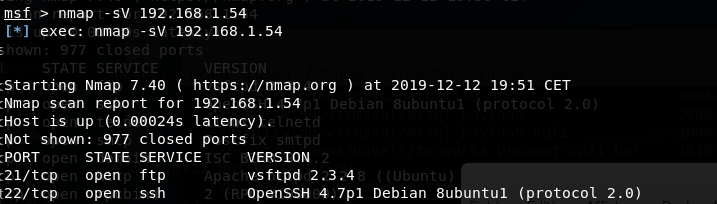
\includegraphics[width=0.75\textwidth]{oui/Screens/nmap.PNG}
  \caption{Utilisation de Nmap}
  \label{fig:courbe-tikz}
\end{figure}
À partir de nmap, on obtient tous les ports ouverts sur la machine distante ainsi que les services qui sont actifs sur cette dernière. Par exemple, dans cette capture le port 22 qui correspond à SSH est ouvert ainsi que le port 80 qui correspond à un serveur HTTP (Apache). Cela veut dire que nous pouvons accéder à un serveur web depuis le navigateur en tapant dans l’URL “http://192.168.1.27”. De plus, nous pouvons nous connecter au serveur SSH sous réserve d’avoir des identifiants et un mot de passe. Mais à l’heure actuelle, nous n’avons rien de cela. Tout le but du CTF sera de récupérer ces informations ou de passer par des méthodes tierces dans le but de nous infiltrer dans la machine pour récupérer un ou des flags. Nous allons maintenant introduire les différents outils de scans de vulnérabilités. On appelle cela une récolte d’informations active car nous allons entrer directement en relation avec la cible afin d’obtenir des informations utilisables. Tandis qu’une récolte d’informations passive consiste à chercher des informations sur la cible directement sur le web avec des outils comme “whois” pour récupérer des adresses IP ou des DNS ou avec “NSLookup” pour interroger un serveur DNS et obtenir des enregistrements sur les différents hôtes qu’il connaît.